
\documentclass[t]{beamer}  % [t], [c], или [b] --- вертикальное выравнивание на слайдах (верх, центр, низ)
%\documentclass[handout]{beamer} % Раздаточный материал (на слайдах всё сразу)
%\documentclass[aspectratio=169]{beamer} % Соотношение сторон

\usetheme{Pittsburgh} 

\usecolortheme{rose} 

%%% Работа с русским языком
\usepackage{cmap}					% поиск в PDF
\usepackage{mathtext} 				% русские буквы в формулах
\usepackage[T2A]{fontenc}			% кодировка
\usepackage[utf8]{inputenc}			% кодировка исходного текста
\usepackage[english,russian]{babel}	% локализация и переносы

%% Beamer по-русски
\newtheorem{rtheorem}{Теорема}
\newtheorem{rproof}{Доказательство}
\newtheorem{rexample}{Пример}

%%% Дополнительная работа с математикой
\usepackage{amsmath,amsfonts,amssymb,amsthm,mathtools} % AMS
\usepackage{icomma} % "Умная" запятая: $0,2$ --- число, $0, 2$ --- перечисление

%% Номера формул
%\mathtoolsset{showonlyrefs=true} % Показывать номера только у тех формул, на которые есть \eqref{} в тексте.
%\usepackage{leqno} % Нумерация формул слева

%% Свои команды
\DeclareMathOperator{\sgn}{\mathop{sgn}}

%% Перенос знаков в формулах (по Львовскому)
\newcommand*{\hm}[1]{#1\nobreak\discretionary{}
	{\hbox{$\mathsurround=0pt #1$}}{}}

%%% Работа с картинками
\usepackage{graphicx}  % Для вставки рисунков
\graphicspath{{images/}}  % папки с картинками
\setlength\fboxsep{3pt} % Отступ рамки \fbox{} от рисунка
\setlength\fboxrule{1pt} % Толщина линий рамки \fbox{}
\usepackage{wrapfig} % Обтекание рисунков текстом

%%% Работа с таблицами
\usepackage{array,tabularx,tabulary,booktabs} % Дополнительная работа с таблицами
\usepackage{longtable}  % Длинные таблицы
\usepackage{multirow} % Слияние строк в таблице

%%% Программирование
\usepackage{etoolbox} % логические операторы

%%% Другие пакеты
\usepackage{lastpage} % Узнать, сколько всего страниц в документе.
\usepackage{soul} % Модификаторы начертания
\usepackage{csquotes} % Еще инструменты для ссылок
%\usepackage[style=authoryear,maxcitenames=2,backend=biber,sorting=nty]{biblatex}
\usepackage{multicol} % Несколько колонок

%%% Картинки
\usepackage{tikz} % Работа с графикой
\usepackage{pgfplots}
\usepackage{pgfplotstable}



\title{Идеальный ужин: рецепты приготовления}
\subtitle{Практическое задание}
\author{Крафт Ярослав}
\date{\today}


\begin{document}

\frame[plain]{\titlepage}
		
\begin{frame} \label{begin} % Первый фрейм
	Каждая хозяйка, хотя бы раз в неделю, но задается вопросом что приготовить на ужин. Хочется разнообразия, чего--то нового, но вот экспериментировать и часами готовить неизвестное блюдо нет особого желания. В таким моменты выручат всем известные, но забытые блюда.	
\end{frame}
	
\section{Сытная}
\begin{frame}  % Второй фрейм
\frametitle{\insertsection}
	Сытная и безумно вкусная запеканка, состоящая из фарша, картофеля и помидоров, способна поднять настроение и зарядить энергией. Блюдо готовится очень просто и достаточно быстро. Запеканкой можно порадовать домочадцев и удивить внезапных гостей. \pause
		
	\textbf{Необходимые для приготовления ингредиенты:}
	\begin{multicols}{2}
		\begin{itemize}
			\item Фарш свиной --- 500~гр.;
			\item Куриное яйцо --- 2~шт.;
			\item Картофель --- 900~гр.;  
			\item Помидор --- 200~гр.;
			\item Репчатый лук --- 150~гр.;
			\item Твердый сыр --- 350~гр.;
			\item Майонез --- 75~гр.;
			\item Сметана --- 75~гр.;
			\item Соль;
			\item Черный молотый перец;
			\item Растительное масло.
		\end{itemize}	
	\end{multicols}
\end{frame}

\section{Последовательность приготовления}
\begin{frame} % Третий фрейм
\frametitle{\insertsection}
	\only<1>{
	\begin{enumerate}
		\item Фарш лучше приготовить самостоятельно. Для этого необходимо взять свиную мякоть, удалить с мяса лишний жир, нарезать небольшими кусочками. Пропустить мясо через мясорубку или измельчить при помощи кухонного комбайна.
		\item К готовому свиному фаршу добавить сырые куриные яйца, соль и перец. Перемешать до получения однородной консистенции.
		\item Картофель почистить от кожуры, помыть и нарезать кружочками.	 
		\item Форму для запекания щедро смазать маслом и равномерно выложить картофельные кружочки. Посолить картофель по вкусу.
	\end{enumerate}
	}
	\only<2>{
	\begin{enumerate}
		\setcounter{enumi}{4}
		\item Приготовить соус. Для этого необходимо смешать майонез и сметану, добавить любимые специи и немного соли, а также 70~миллилитров чистой воды. Перемешать до однородности. Чтобы блюдо было более пикантным можно добавить немного горчицы.
		\item Полученным соусом полить картофель. Тогда он быстрее приготовится, будет сочным и мягким.
		\item Репчатый лук очистить от шелухи и нарезать полукольцами.
		\item Равномерно распределить нарезанный лук по всей поверхности картофеля.
	\end{enumerate}
	}
	\only<3>{
	\begin{enumerate}
		\setcounter{enumi}{8}
		\item На репчатый лук сверху выложить свиной фарш. Аккуратно разровнять его и распределить, чтобы мясо было по всей поверхности запеканки.
		\item Свежие помидоры промыть и нарезать тонкими кольцами. Выложить их на фарш. Кольца выкладывать внахлест друг на друга.
		\item Помидоры смазать майонезом.
		\item Твердый сыр натереть на крупной терке. Посыпать им запеканку.
		\item Выпекать блюдо в духовке, разогретой до 180~градусов, 40--45~минут.	
	\end{enumerate}
	}
	\only<4>{
	При желании в запеканку можно добавить крупно нарезанные шампиньоны. Грибы сделают вкус блюда особенным. Запеканка --- это самостоятельное блюдо, которое не нуждается в дополнениях.
	\begin{center}
		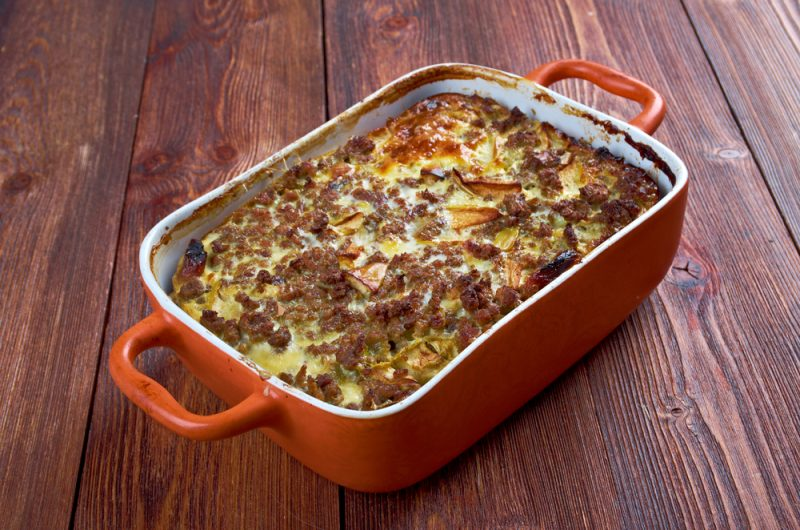
\includegraphics[height=5cm, keepaspectratio]{1}
	\end{center}
	}
\end{frame}

\section{Итальянец}
\begin{frame} % Четвертый фрейм
	\frametitle{\insertsection}
	Спагетти --- это уже настолько привычное блюдо, что удивить им кажется невозможным. Но достаточно немного фантазии и спагетти станут частым гостем на повседневном столе. Одно из главных достоинств рецепта заключается в том. что он очень быстрый. Пока спагетти варятся мясной соус к ним будет уже готов. \pause
	
	\textbf{Необходимые для приготовления ингредиенты:}
	\begin{multicols}{2}
		\begin{itemize}
			\item Спагетти --- 250~гр.;
			\item Куриное филе --- 500~гр.;
			\item Помидоры черри --- 300~гр.;
			\item Сыр чеддер --- 150~гр.;
			\item Чеснок --- 3 зубчика;
			\item Черный молотый перец;
			\item Соль;
			\item Растительное масло.
		\end{itemize}	
	\end{multicols}
\end{frame}	

\section{Последовательность приготовления}
\begin{frame} % Пятый фрейм
	\frametitle{\insertsection}
	\only<1>{
		\begin{enumerate}
			\item В широкую кастрюлю налить воды, довести до кипения и подсолить.
			\item Добавить в кипящую воду спагетти и варить до готовности, как указано на упаковке. Спагетти необходимо время от времени перемешивать.
			\item Пока варятся спагетти приготовить мясной соус. Для этого следует очистить куриное филе от лишнего жира и пленок, нарезать мясо птицы кубиками небольшого размера.
			\item В сковороду добавить растительное масло, разогреть.Обжарить филе до золотистой корочки.
		\end{enumerate}
	}
	\only<2>{
		\begin{enumerate}
			\setcounter{enumi}{4}
			\item Готовое филе убрать в другую посуду, а в сковороду на которой оно жарилось поместить помидоры черри, предварительно разрезанные напополам.
			\item Чеснок очистить от шелухи. Зубчики пропустить через пресс или мелко нарезать ножом, добавить к помидорам.
			\item К помидорам с чесноком добавить куриное филе и перемешать. Огонь убавить до минимума.
			\item К этому моменту спагетти будут полностью готовы, но прежде, чем их слить на дуршлаг 100~миллилитров воды, в которой они варились, добавить в сковороду к помидорам и куриному филе.
		\end{enumerate}
	}
	\only<3>{
		\begin{enumerate}
			\setcounter{enumi}{8}
			\item Спагетти промыть под холодной водой. Делается это для того,чтобы остановить процесс приготовления, так как горячие спагетти продолжают готовиться под действием собственной температуры.
			\item Промытые спагетти добавить в сковороду к курице и томатам. Перемешать, чтобы соус равномерно распределился. При необходимости посолить и поперчить блюдо.
			\item Сыр натереть на крупной терке.
			\item Спагетти разложить по порциям, сверху присыпать сыром и перемешать.
			\item Петрушку мелко нашинковать и украсить ею готовое блюдо.
		\end{enumerate}
	}
	\only<4>{
	Вкус блюда необычный, нежный и тонкий. Оно понравится даже тем, кто не любит спагетти. Потому что очень много соуса, которому помидоры черри придают особенной пикантности. Дополнительно к блюду можно подать салат из овощей с обилием свежей зелени.
	\begin{center}
		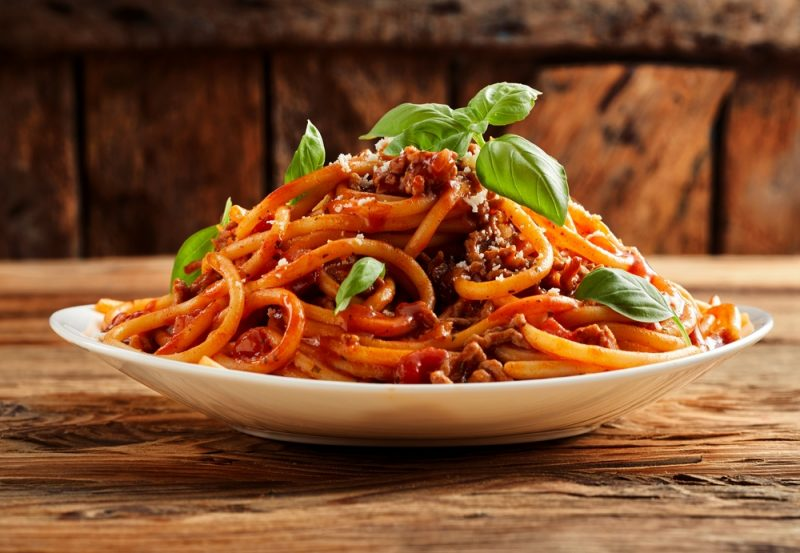
\includegraphics[height=4.5cm, keepaspectratio]{2}
	\end{center}
}
\end{frame}

\if 0 % Многострочный комментарий
 % Ограничение в шесть фреймов
\section{Поход в лес} 
\begin{frame} % Шестой фрейм
	\frametitle{\insertsection}
	В сентябряе грибники начинают активно собирать опята, заготавливать их на зиму. Почитателей грибов так много не просто так. Опята обладают приятным вкусом и нежным ароматом. Их можно консервировать, готовить с ними супы и каши, вариантов приготовления масса. Еще один вариант вкусно приготовить опята --- потушить с курицей, картофелем и другими овощами в горшочках. \pause
	
	\textbf{Необходимые для приготовления ингредиенты:}
	\begin{multicols}{2}
		\begin{itemize}
			\item Куриное филе --- 450~гр.;
			\item Опята --- 300~гр.;
			\item Твердый сыр --- 250~гр.;
			\item Кабачок --- 150~гр.;
			\item Картофель --- 600~гр.;
			\item Репчатый лук --- 100~гр.;
			\item Сливки 20--35~\% --- 170~мл.;
			\item Растительное масло;
			\item Соль.
		\end{itemize}	
	\end{multicols}
\end{frame}	

\section{Последовательность приготовления} 
\begin{frame} % Седьмой фрейм
	\frametitle{\insertsection}
	\only<1>{
		\begin{enumerate}
			\item Репчатый лук очистить от шелухи и нарезать мелкими кубиками.
			\item Разогреть сковороду, добавить растительное масло. Обжаривать лук на растительном масле до того момента, как он не станет прозрачным.
			\item Пока обжаривается лук промыть куриное филе, удалить пленочки и лишний жир, нарезать мясо птицы кубиками небольшого размера.
			\item К луку добавить куриное филе и обжаривать до готовности, помешивая время от времени.
		\end{enumerate}
	}
	\only<2>{
		\begin{enumerate}
			\setcounter{enumi}{4}
			\item Опята сначала отварить, а потом обжарить до готовности на растительном масле. В сковороду к опятам добавить сливки, перемешать и хорошенько посолить. Протушить 7--10~минут. 
			\item Картофель и кабачок очистить от кожуры, нарезать небольшими кубиками.
			В горшочек сначала поместить картофель и кабачок, затем курицу, обжаренную с репчатым луком, затем грибы со сливками. Верхний слой --- это тертый или нарезанный кубиками твердый сыр, который создаст аппетитную золотистую корочку. Добавить в горшочек еще 70--100~миллилитров чистой воды.
			\item Запекать в духовке 35--40 минут при 180~градусах.
		\end{enumerate}
	}
	\only<3>{
		Горшочки необходимо ставить в холодную духовку, чтобы разогревались они постепенно и не лопнули от сильного перепада температур.
		\begin{center}
			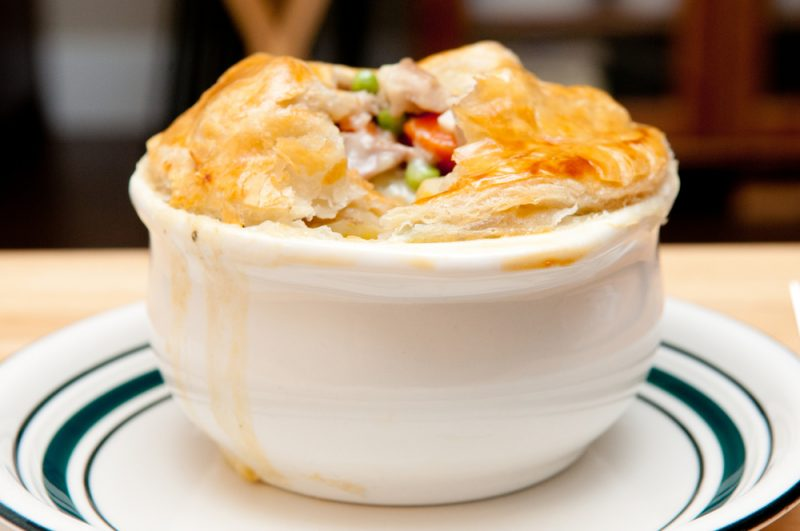
\includegraphics[height=5cm, keepaspectratio]{3}
		\end{center}
	}
\end{frame}

\section{Объедение} 
\begin{frame} % Восьмой фрейм
	\frametitle{\insertsection}
	Гнезда из макарон легко найти на прилавках в магазинах, но что с ними приготовить придумать сложно. Самый простой и беспроигрышный вариант – наполнить мясным фаршем. \pause
	
	\textbf{Необходимые для приготовления ингредиенты:}
	\begin{multicols}{2}
		\begin{itemize}
			\item Свино--говяжий фарш --- 350~гр.;
			\item Томатный сок --- 250~мл.;
			\item Гнезда из макарон --- 8~шт.;
			\item Репчатый лук --- 120~гр.;
			\item Растительное масло --- 50~мл.;
			\item Томатная паста --- 40~гр.;
			\item Укроп --- 1 пучок;
			\item Соль;
			\item Молотый черный перец.
		\end{itemize}	
	\end{multicols}
\end{frame}	

\section{Последовательность приготовления}
\begin{frame} % Девятый фрейм
	\frametitle{\insertsection}
	\only<1>{
		\begin{enumerate}
			\item Лук почистить от шелухи и нарезать небольшими кубиками.
			\item В глубокую тарелку положить фарш, добавить лук, соль и перец. Перемешать для того, чтобы лук и специи в фарше равномерно распределились.
			\item Гнезда из макарон важно подбирать примерно одного размера и диаметра.
			\item Выложить их в широкую сковороду с высокими бортиками.
			\item В серединку каждого гнезда поместить несколько ложек свино-говяжьего фарша, чтобы они были плотно и равномерно наполнены.
		\end{enumerate}
	}
	\only<2>{
		\begin{enumerate}
			\setcounter{enumi}{5}	
			\item В отдельной посуде смешать масло, томатную пасту и соль. Перемешать до однородной консистенции. Добавить томатный сок и еще раз перемешать до полного растворения томатной пасты. Попробовать соус, при необходимости добавить немного сахара, соли или перца. 
			\item Гнезда, наполненные фаршем, залить томатным соусом.
			\item Сковороду с блюдом закрыть крышкой и переместить на средний огонь. Готовить гнезда с фаршем 25--30~минут до полной готовности. 
			\item Укроп мелко нашинковать и посыпать зеленью готовые гнезда. Можно подавать к столу.
		\end{enumerate}
	}
	\only<3>{
		Даже из простейших ингредиентов всегда найдется, что приготовить вкусного и необычного. При правильном подходе готовка не займет много времени и процесс принесет массу удовольствия, как и готовые блюда.
		\begin{center}
			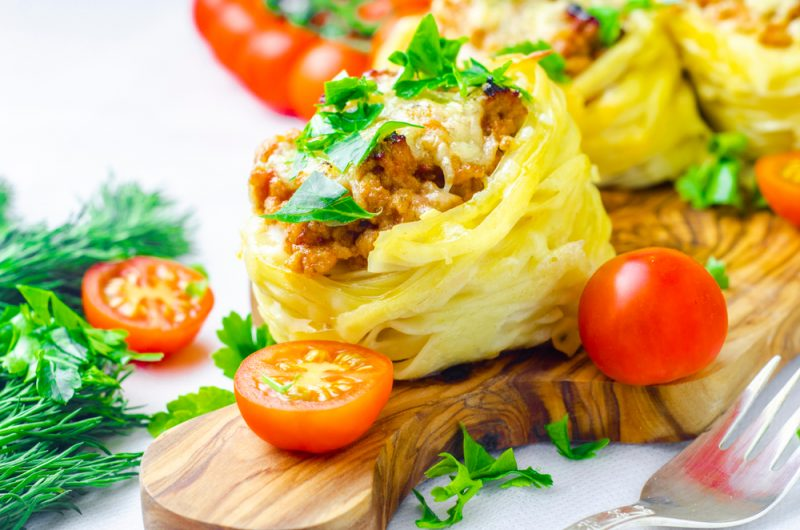
\includegraphics[height=5cm, keepaspectratio]{4}
		\end{center}
	}
\end{frame}	
\fi % Конец комментария

\section{Авторство материалов}	
\begin{frame} % Десятый фрейм
	\frametitle{\insertsection}	
	Использованы материалы статьи ,,Идеальный ужин: рецепты приготовления'', опубликованной на сайте 
	 \color [RGB]{0,0,255} \href{https://www.chefmarket.ru/blog/idealnyj-uzhin-recepty-prigotovlenija/}{Шефмаркет} \color [RGB]{0,0,0} 13.08.2019~г.
	\begin{center}
		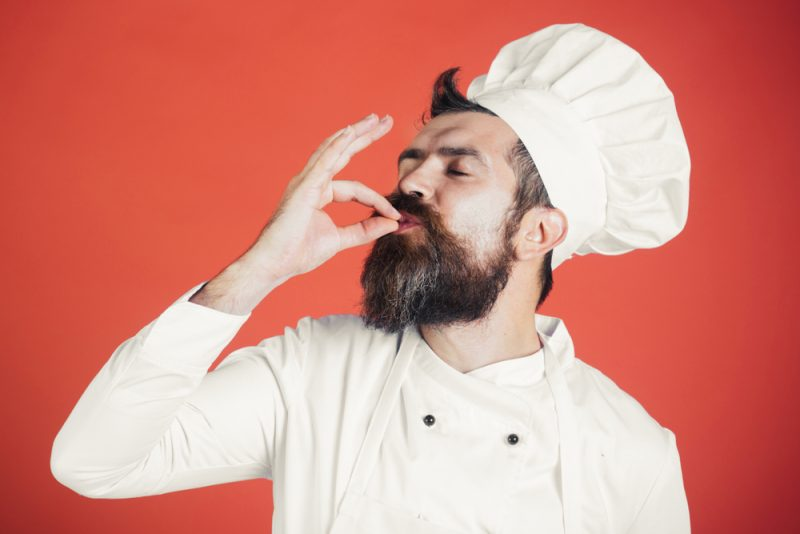
\includegraphics[height=5cm, keepaspectratio]{5}
	\end{center}
	\begin{block}{}
		\hyperlink{begin}{\beamerbutton{Возвращение в начало презентации}} 
	\end{block}
\end{frame}
	
	
\end{document}
